\begin{task}{2, Diffusion Maps}
\paragraph{Implementation}
For this task, the model was implemented in \verb|diffusion_maps/model.py| and python notebooks for the following tests can be found in the same folder. The \verb|fit(...)| function takes the input data and a \verb|max_dist| for the distance matrix. In the implementation of the diffusion map we purely follow the efficient approach outlined in the exercise sheet. Therefore the \verb|max_dist| argument is for calculating neighbors efficiently using \verb|KDTree| from \verb|scipy|. Also, we used sparse matrices whenever possible to get better performance.

The exercise description recommends using an efficient implementation using sparse matrices and only considering points within a reasonable neighborhood for calculating the distance matrix. During testing it turned out that considering more points leads to better results in general, hence \verb|max_dist| was set to consider all points. Further details will be discussed in each section.

Note that according to \cite{berry2013} $\alpha =1$ the resulting diffusion map is the Laplace-Beltrami operator. The diffusion map is created according to step 19 in the algorithm from \cite{berry2013} with the timescale fixed to $t=1$. In our implementation, the $\phi_0$ is not included in the diffusion map. Formally we compute our diffusion map embedding using the following expression:

\begin{align}
    \Phi_{\alpha =1, t=1}(x_i)=\left[ \lambda_1^t\phi_1 (x_i ),...,\lambda_L^t\phi_L (x_i )\right] ^T \label{diffmap}
\end{align}

A keen reader would have seen that the exercise sheet outlines the same formula for the Laplace-Beltrami operator using this expression:
\begin{align*}
    \Delta\phi_k = \lambda_k\phi_k ,\qquad k\in\mathbb{N}
\end{align*}

The following tests can be reproduced in the python notebooks, see \verb|Exercise-3/README.md| for further clarification.

%%%%%%%%%%%%%%%%%%%%%%%%%%%%%%%%%%%%%%%%%%%%%%%%%%
%%%%%%%%%% PART 1
%%%%%%%%%%%%%%%%%%%%%%%%%%%%%%%%%%%%%%%%%%%%%%%%%%
\paragraph{1.1: Demonstrate similarity between Diffusion Map and Fourier Analysis}
In the first part we want to demonstrate the similarity between Diffusion Maps and Fourier Analysis. To do this we computed the first 5 eigenfunctions $\phi_l$ corresponding to the largest eigenvalues $\lambda_l$ using Diffusion Maps on a data set with $N=1000$ points. The data set is given by:
\begin{align*}
    X &= \{ x_k\in\mathbb{R}^2\}^N_{k=1}\\
    x_k &= (\text{cos}(t_k), \text{sin}(t_k))\\
    t_k &=  (2\pi k)/(N+1)
\end{align*}
A plot of the first five eigenfunctions $\phi_l$ can be found in Figures \ref{fig:t2_1-dmapAll} and \ref{fig:t2_1-dmapSeparate}.

The initial dataset is visualized in Figure \ref{fig:t2_1-dmapAll}(a). The generated data contains a tuple with coordinates for one period of the $sin$- and $cos$-function. In Figure \ref{fig:t2_1-dmapAll}(b) we plotted all eigenfunctions $\phi_l$ against $t_k$, while a separate Figure of each eigenfunction (from the diffusion map embedding) can be found in Figures \ref{fig:t2_1-dmapSeparate}. Here we can see $\phi_1$ and $\phi_2$ reconstruct the $sin$- and $cos$-functions respectively. $\phi_3$ and $\phi_4$ contain 2 periods of the $sin$- and $cos$-function, but shifted by a phase of $period/2$. We can observe in $\phi_5$ 3 periods of the $sin$-function (with a phase-shift of $period/2$) and assume that with increasing $l$ of the eigenfunctions $\phi_l$ more periods are squeezed into the window given by the $t_k$.

Before comparing the eigenfunctions $\phi_l$ with the Diffusion Map coordinates, it is important to note that running the experiment can result in phase shifts of $period/2$ for each $\phi_l$. So for example $\phi_1$ was sometimes the $-sin()$-function. Secondly, the initial testing was done with \verb|max_dist=1.0| for the distance matrix. This led to the calculation an embedding with $sin$- and $cos$-functions of higher frequencies. All presented results were calculated with \verb|max_dist=9.0| which takes all points into account for calculating the distance matrix.

Next in Figure \ref{fig:t2_1-dmapAll}(d) the diffusion map coordinates (see \ref{diffmap}) were plotted against $t_k$. We can observe that between Figures \ref{fig:t2_1-dmapAll} (b) and (d), that amplitudes are scaled down by the corresponding eigenvalues $\lambda_l$. We conclude the eigenvalues $\lambda_l$ could describe the importance of each eigenfunction $\phi_l$. In the following section whenever we mention the eigenfunction $\phi_l$ it refers to the diffusion map embedding (see \ref{diffmap}).

Further observations of $\phi_l$ for large $l$ leads to the assumption that $\phi_l$ for $l\in\mathbb{N}$ represents the $sin$- and $cos$-functions correspondingly at higher frequencies (disregarding the phase-shift of $period/2$). It is also notable when \verb|max_dist| is low that a sparser distance matrix causes an increase of the initial frequency observed in $\phi_1$.

\begin{figure}[H]
\centering
\subfigure[Fourier data set]{
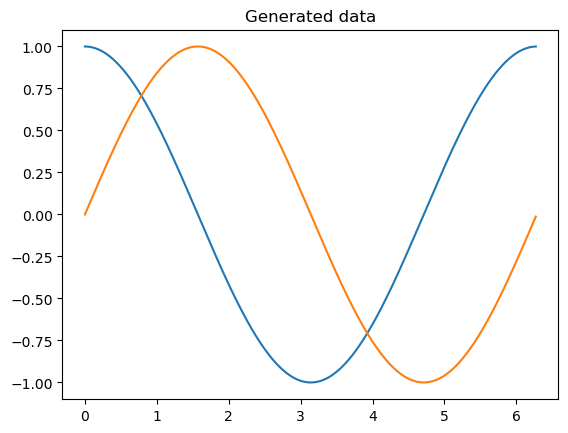
\includegraphics[width=0.35\textwidth]{images_task2/t2_1-fourier.png}}
\subfigure[All eigenfunctions $\phi_l$]{
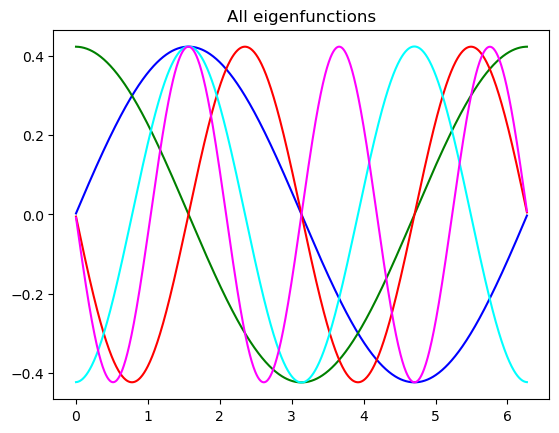
\includegraphics[width=0.35\textwidth]{images_task2/t2_1-allPhis.png}}
\subfigure[Comparison of diffusion map functions]{
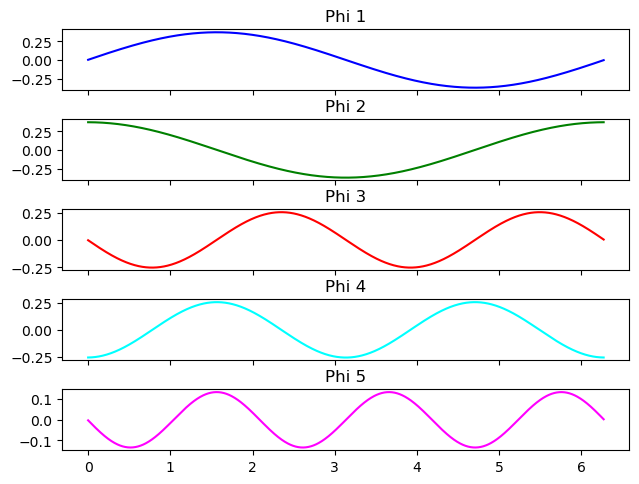
\includegraphics[width=0.35\textwidth]{images_task2/t2_1-compareDmap.png}}
\subfigure[All diffusion map functions]{
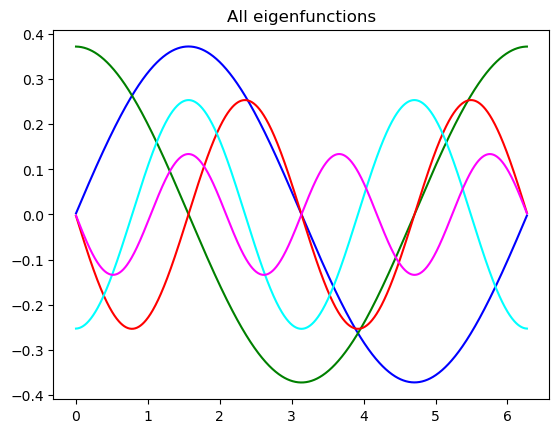
\includegraphics[width=0.35\textwidth]{images_task2/t2_1-allDmaps.png}}
\caption{Diffusion Map results}
\label{fig:t2_1-dmapAll}
\end{figure}

\begin{figure}[H]
\centering
\subfigure[$\phi_1$]{
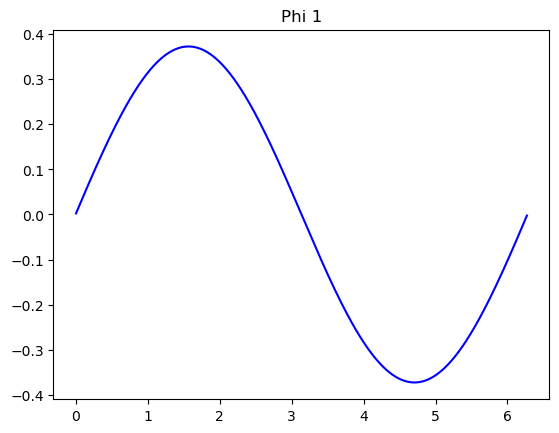
\includegraphics[width=0.3\textwidth]{images_task2/t2_1-phi1.png}}
\subfigure[$\phi_2$]{
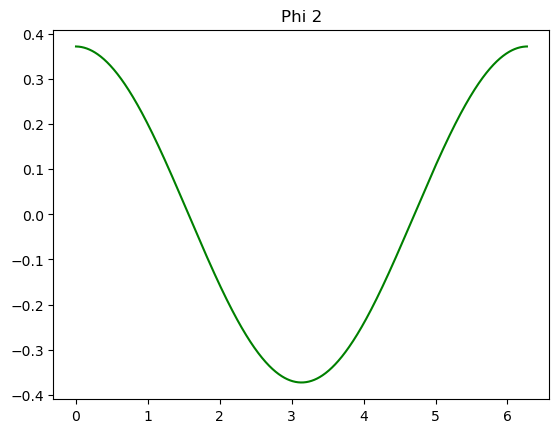
\includegraphics[width=0.3\textwidth]{images_task2/t2_1-phi2.png}}
\subfigure[$\phi_3$]{
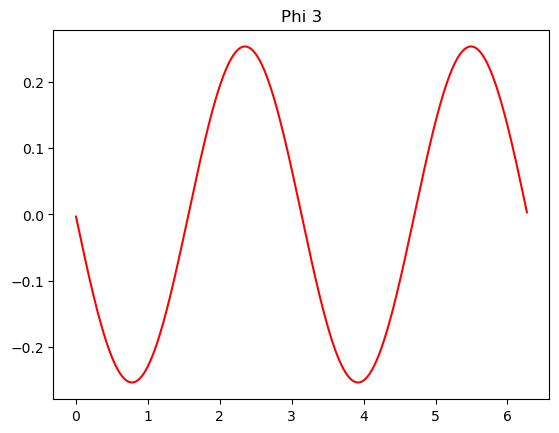
\includegraphics[width=0.3\textwidth]{images_task2/t2_1-phi3.png}}
\subfigure[$\phi_4$]{
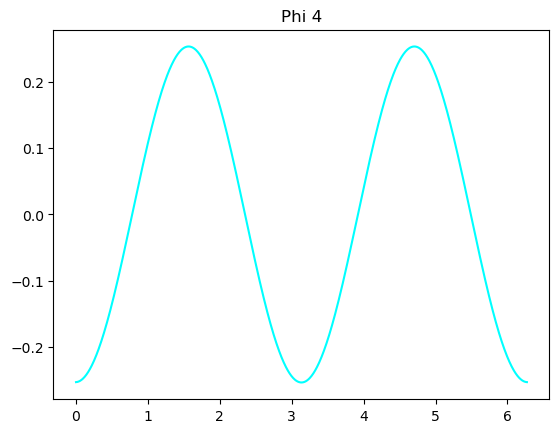
\includegraphics[width=0.3\textwidth]{images_task2/t2_1-phi4.png}}
\subfigure[$\phi_5$]{
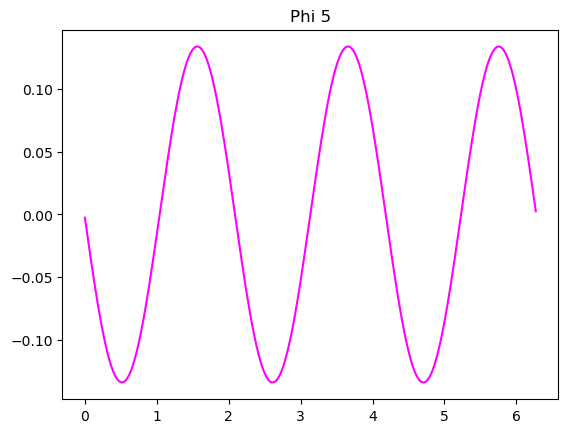
\includegraphics[width=0.3\textwidth]{images_task2/t2_1-phi5.png}}
\caption{Separate Diffusion Map results}
\label{fig:t2_1-dmapSeparate}
\end{figure}

\paragraph{1.2: Bonus}
We see that the diffusion map can perfectly replicate the input data, as $\phi_1$ and $\phi_2$ represent the input data perfectly when disregarding the phase-shift. We can confirm this observation by plotting the input data as $(x_1 ,x_2$ and then comparing it to the diffusion map embedding $(\phi_1 ,\phi_2 )$. In figure \ref{fig:t2_1-dmapDifferent} we observe that the manifold of the input data is perfectly captured by the diffusion map.

\begin{figure}[H]
\centering
\subfigure[Plot $x_1$ against $x_2$]{
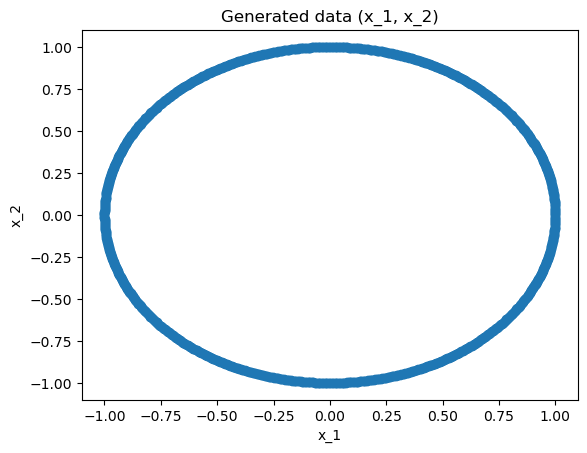
\includegraphics[width=0.45\textwidth]{images_task2/t2_1-datax1x2.png}}
\subfigure[Plot $\phi_1$ against $\phi_k$, $k\in\{ 2,3,4,5\}$]{
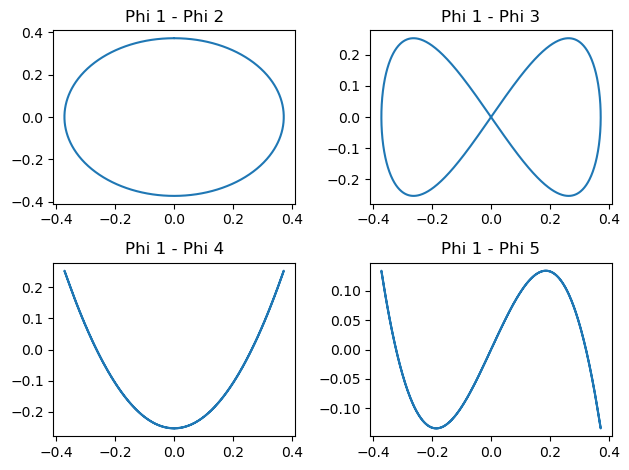
\includegraphics[width=0.45\textwidth]{images_task2/t2_1-phis.png}}
\caption{Different plots of Fourier data}
\label{fig:t2_1-dmapDifferent}
\end{figure}

%%%%%%%%%%%%%%%%%%%%%%%%%%%%%%%%%%%%%%%%%%%%%%%%%%
%%%%%%%%%% PART 2
%%%%%%%%%%%%%%%%%%%%%%%%%%%%%%%%%%%%%%%%%%%%%%%%%%
\paragraph{2: The "Swiss Roll" data set}
In the second part we want to use the algorithm to obtain the first 10 eigenfunctions of the Laplace-Beltrami operator on the "swiss roll"-manifold. The data points $u_k$ and $v_k$ are sampled uniformly at random and define data set as follows:
\begin{align*}
    X &= \{ x_k\in\mathbb{R}^3\}^N_{k=1}\\
    x_k &= (u_k\text{cos}(u_k), v_k, u_k\text{sin}(t_k))\\
    u_k &\in \left[ 3/2\pi ,3\pi\right]\\
    v_k &\in \left[ 0, 21\right]
\end{align*}
In the following experiment all data points were sampled using the \verb|sklearn| library function:
\begin{center}
    \verb|sklearn.datatsets.make_swiss_roll(...)|.    
\end{center}
The function argument \verb|random_state=69| was set to have reproducible results. Also \verb|sklearn| outputs an additional vector containing the univariate position of the sample according to the main dimension of the points in the manifold. This allows us to visualize the data points colored according to their univariate position. Hence we did not use our own implementation for creating sample points.

The experiment was performed with setting \verb|max_dist=60.0|. Considering to few neighbors for the distance matrix leads to similar results as having little amounts of sampling data. Also note that due to points being sampled at random, the points are presented using a scatter plot.

\paragraph{2.1: 3D plot of "swiss roll"}
In figure \ref{fig:t2_2-swissroll} we see a 3D plot of the "swiss roll" data set with $N=5000$ sampled points. 

\begin{figure}[H]
\centering
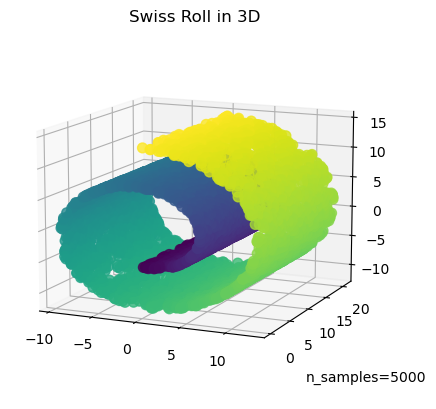
\includegraphics[width=0.5\textwidth]{images_task2/t2_2-swissroll5k.png}
\caption{Swiss Roll with $N=5000$ sample points}
\label{fig:t2_2-swissroll}
\end{figure}

\paragraph{2.2: 10 eigenfunctions on swiss roll plotted on $\phi_1$}
Obviously $\phi_1$ plotted against itself will show the linear function $f(x) = x$, hence we excluded this plot. In Figure \ref{fig:t2_2-phis5k} we see $\phi_1$ plotted against $\phi_2$ to $\phi_{10}$. We see that for the first 3 subplots with $l\leq 4$ the results look like polynomial functions of degree 2, 3 and 4. Clearly "swiss-roll" is unrolled, but the sample points were mapped into a 1D space.

\paragraph{2.3: Number of $l$ eigenfunctions where $\phi_l$ is no longer a function of $\phi_1$?}
For $l=5$ in the subplot "Phi 1 - Phi 5" we observe the "swiss-roll"-manifold unrolled as a plane in a 2d-space and $\phi_5$ is no longer a function of $\phi_1$. For $l>4$ we see further attempts at unrolling appear in the next few scatter plots except for "Phi 1 - Phi 8". We observe that for higher $l$ the diffusion map embedding has an linear increase in "knots".
\begin{figure}[H]
\centering
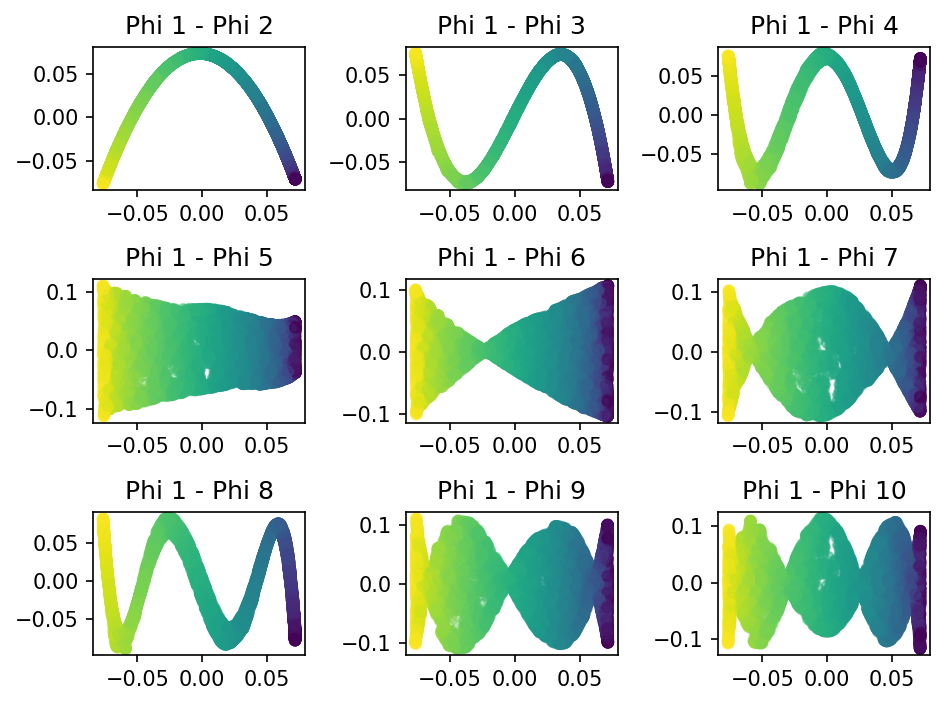
\includegraphics[width=0.7\textwidth]{images_task2/t2_2-scatterplot5k.png}
\caption{Scatter plot results}
\label{fig:t2_2-phis5k}
\end{figure}

\paragraph{2.3: PCA on "swiss roll" with $N=5000$}
Next we used PCA with 3 and 2 components on the "swiss roll" data set for $N=5000$ sample points. In Figure \ref{fig:t2_2-pca5k} we see that 3 components can perfectly capture "swiss roll", but 2 components are only able to capture a 2 dimensional projection of the "swiss roll".

\paragraph{2.4: Why do you need 3 principal components for the swissroll, not 2?}
The "swiss roll" is a 3-dimensional object and has variances in all 3 dimensions. Since PCA can neither discover nor make use of the 2 dimensional manifold of the "swiss roll", therefore, needs 3 components to reconstruct it.

\begin{figure}[H]
\centering
\subfigure[PCA with 3 components]{
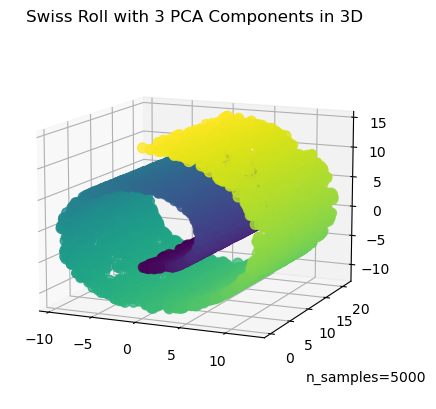
\includegraphics[width=0.42\textwidth]{images_task2/t2_2-pca5k3c.png}}
\subfigure[PCA with 2 components]{
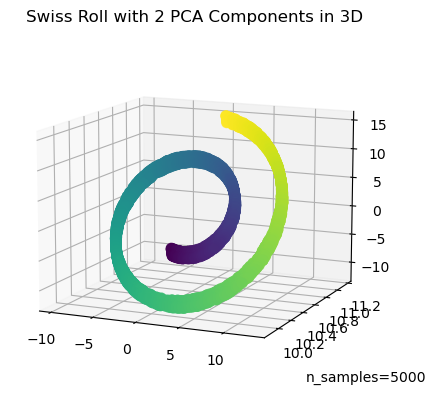
\includegraphics[width=0.42\textwidth]{images_task2/t2_2-pca5k2c.png}}
\caption{PCA on "swiss roll"  with $N=5000$ sampled points}
\label{fig:t2_2-pca5k}
\end{figure}

\paragraph{2.5: Diffusion Map on"Swiss Roll" with $N=1000$}
In this section, we repeat the previous experiment with fewer sample points $N=1000$. In Figure \ref{fig:t2_2-swissroll1k} we see again a 3D plot of the "swiss roll" with $N=1000$ sampled points. Comparing it to the "swiss roll" from Figure \ref{fig:t2_2-swissroll} we can clearly see some holes due to having significantly less sample points.
\begin{figure}[H]
\centering
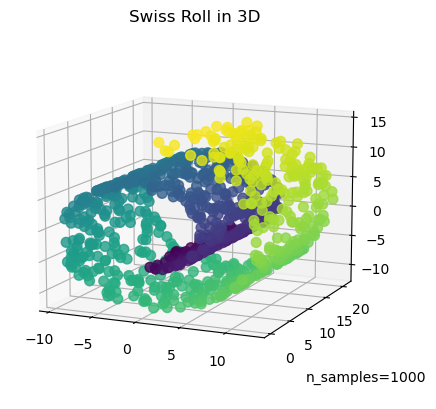
\includegraphics[width=0.5\textwidth]{images_task2/t2_2-swissroll1k.png}
\caption{Swiss Roll with $N=5000$ sample points}
\label{fig:t2_2-swissroll1k}
\end{figure}

In Figure \ref{fig:t2_2-phis1k} we see $\phi_1$ plotted against $\phi_2$ to $\phi_{10}$. Notieably with less sample points the diffusion map embedding degrades in quality. The previously observed functions now look poorly drawn. Also the unrolling we saw in "Phi 1 - Phi 5" can not be observed anymore. Similar results can be seen as well, when setting the \verb|max_dist| for the distance matrix too low. Less data points can lead to different embeddings in the diffusion map. Similar to Fourier data set where we saw phase-shifts in the output, here we observe diffusion map points being mirrored, when comparing to \ref{fig:t2_2-phis5k}.
\begin{figure}[H]
\centering
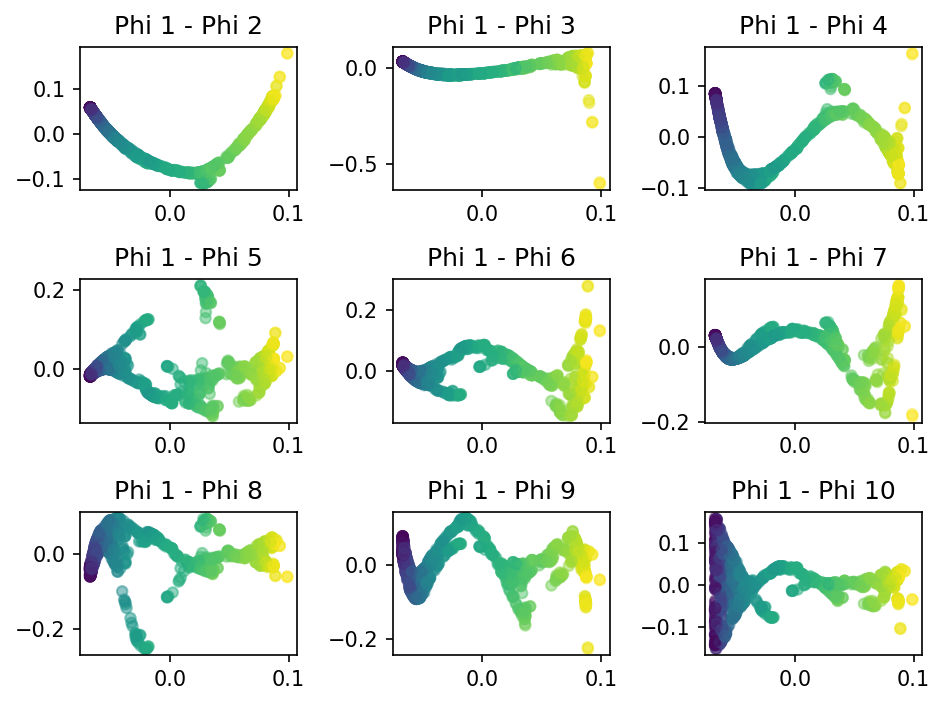
\includegraphics[width=0.7\textwidth]{images_task2/t2_2-scatterplot1k.png}
\caption{Scatter plot results}
\label{fig:t2_2-phis1k}
\end{figure}

\paragraph{2.6: PCA with $N=1000$ samples}
Here we repeat the same experiments on PCA with $N=1000$ samples. In Figure \ref{fig:t2_2-pca1k} we can once again see a good reconstruction using 3 components.  In Figure \ref{fig:t2_2-pca1k}(b) the reconstruction with 2 components looks 3D, but we are actually observing high variance. With less samples, hence a lower confidence for the positions of the data points.
\begin{figure}[H]
\centering
\subfigure[PCA with 3 components]{
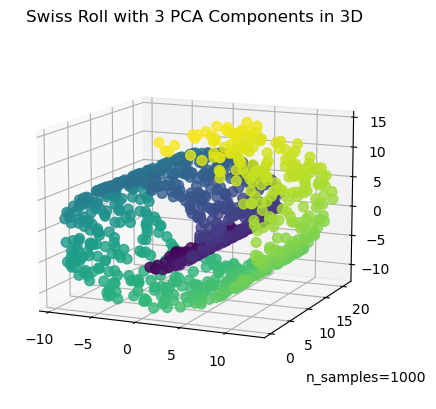
\includegraphics[width=0.42\textwidth]{images_task2/t2_2-pca1k3c.png}}
\subfigure[PCA with 2 components]{
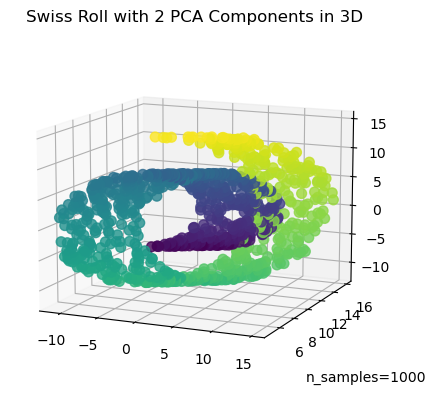
\includegraphics[width=0.42\textwidth]{images_task2/t2_2-pca1k2c.png}}
\caption{PCA on "swiss roll" with $N=1000$ sampled points}
\label{fig:t2_2-pca1k}
\end{figure}

\paragraph{2.7: Bonus - Diffusion Map on "swiss-roll" using \texttt{datafold}}
In this section we applied the diffusion map algorithm provided by the \verb|datafold| library. We used the tutorial python notebook "Diffusion Maps: Embedding of a S-curve manifold" from \url{https://datafold-dev.gitlab.io/datafold/tutorial_03_dmap_scurve.html} as basis. The initial plot \ref{fig:t2_2-bonusA}(a) of of the "swiss-roll" shows 1000 samples of the $N=15000$ sampled points. This library is very efficient an manages to obtain the diffusion map embedding significantly faster than our implementation. Another nice feature of \verb|datafold| is that it can automatically chose an embedding for you as seen in Figure \ref{fig:t2_2-bonusA}(b).
\begin{figure}[H]
\centering
\subfigure["swiss-roll" plot]{
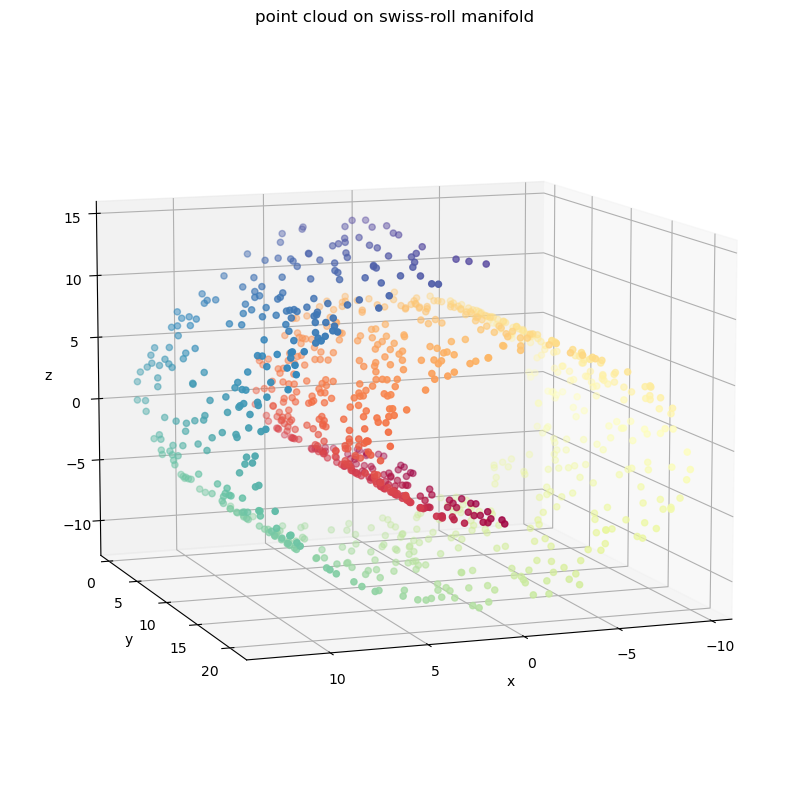
\includegraphics[width=0.35\textwidth]{images_task2/t2_2-bonusSwiss.png}}
\subfigure[Chosen embedding]{
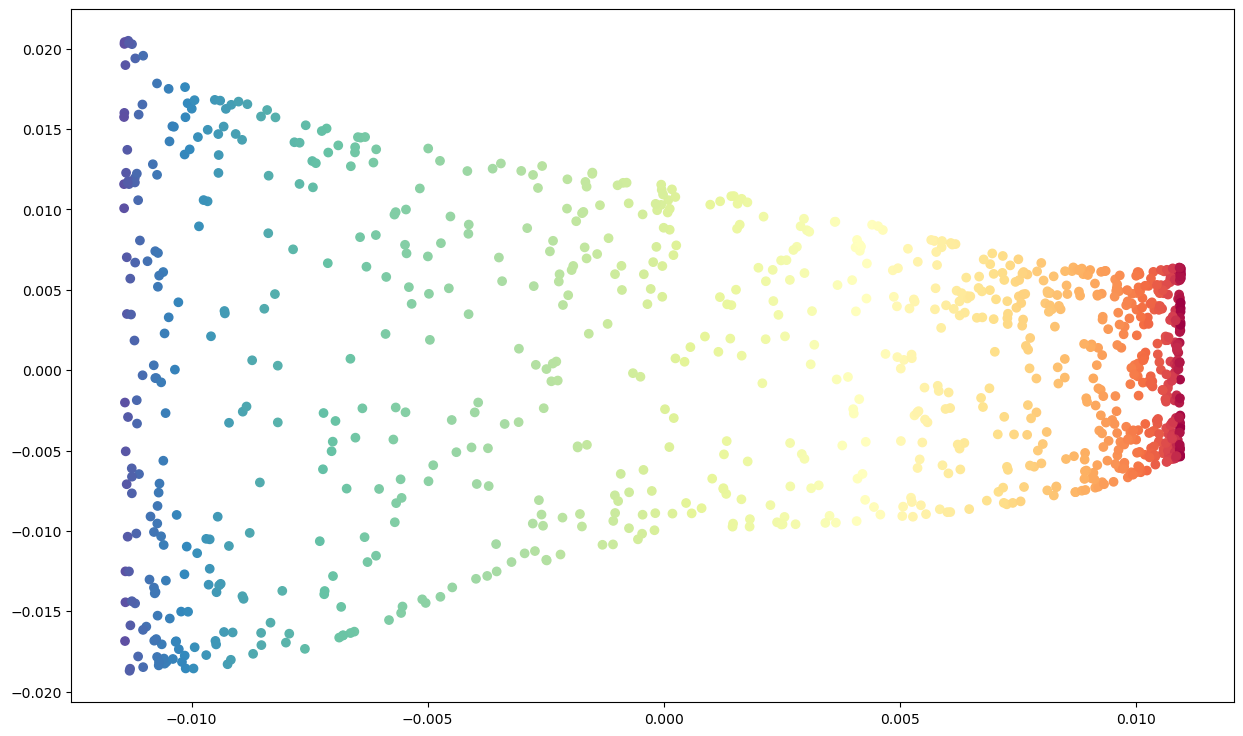
\includegraphics[width=0.35\textwidth]{images_task2/t2_2-bonusChose.png}}
\caption{Diffusion Map using datafold on "swiss roll" with $N=15000$}
\label{fig:t2_2-bonusA}
\end{figure}

In Figure \ref{fig:t2_2-bonusB} we see the first eigenfunctions plotted against other eigenfunctions. Comparing the results to ours from Figure \ref{fig:t2_2-phis5k} we see similar results from the diffusion map from the \verb|datafold| library.
\begin{figure}[H]
\centering
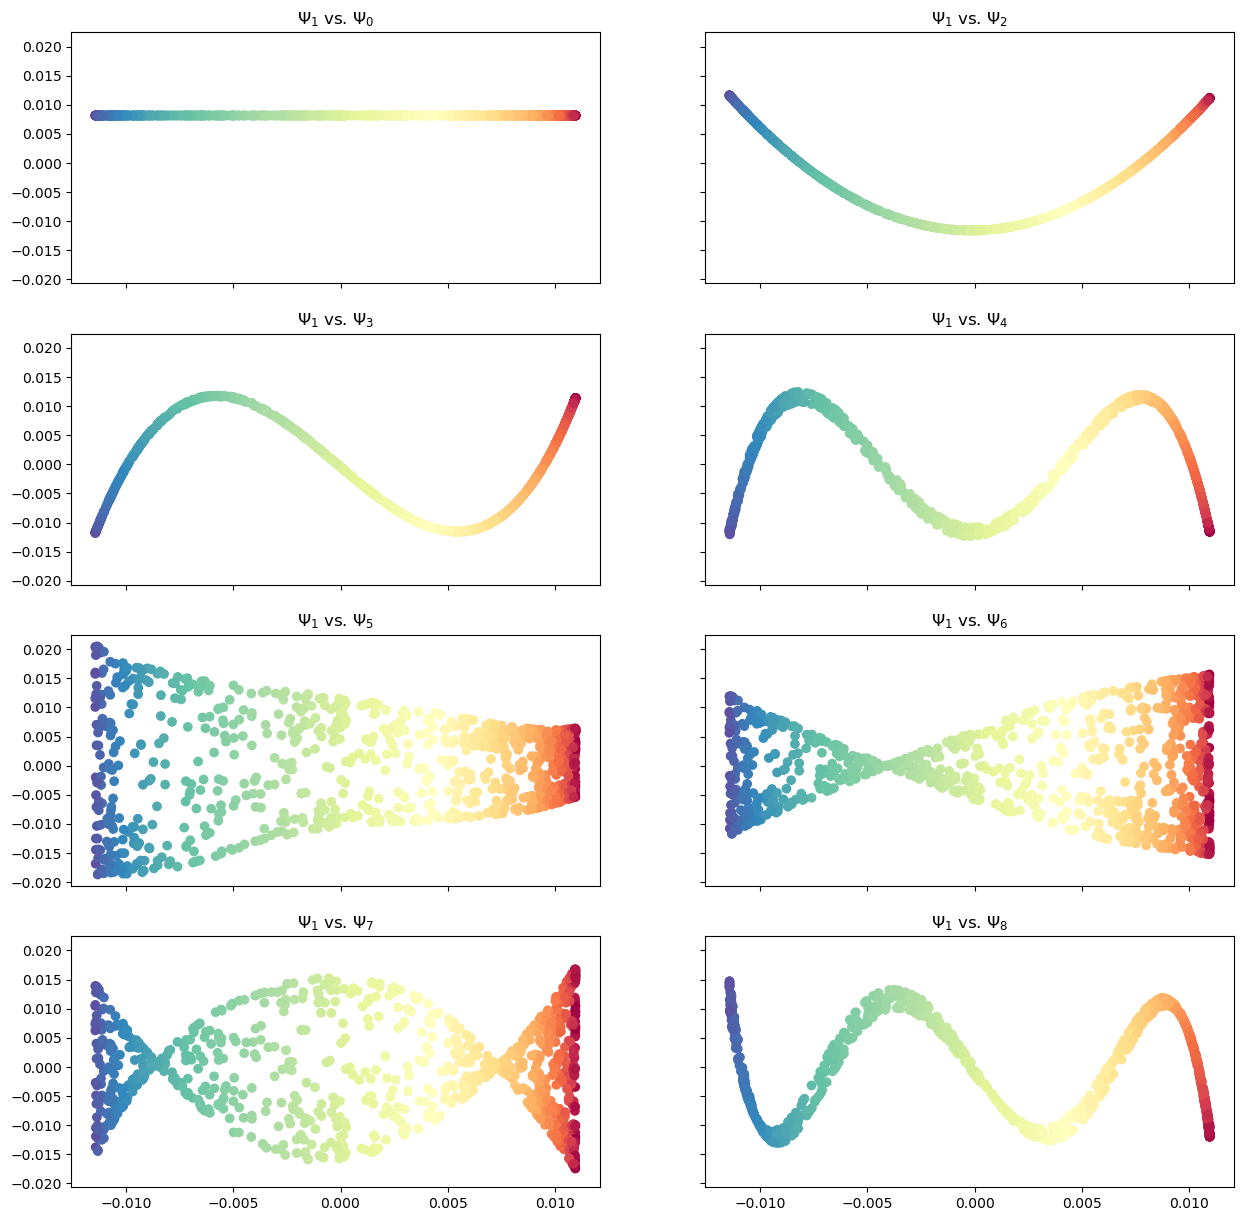
\includegraphics[width=0.6\textwidth]{images_task2/t2_2-bonusPhis.png}
\caption{Plotting the eigenfunction against each other}
\label{fig:t2_2-bonusB}
\end{figure}

%%%%%%%%%%%%%%%%%%%%%%%%%%%%%%%%%%%%%%%%%%%%%%%%%%
%%%%%%%%%% PART 3
%%%%%%%%%%%%%%%%%%%%%%%%%%%%%%%%%%%%%%%%%%%%%%%%%%
\paragraph{3: The Vadere dataset}
In this part we want to perform the same analysis as we did in the previous section with PCA. Once again we have plotted all pedestrian trajectories in Figure \ref{fig:t2_3-allTraj}. We can see that all pedestrians are walking around in a circle. This already tells us that the diffusion map embedding should be an ellipse.
\begin{figure}[H]
\centering
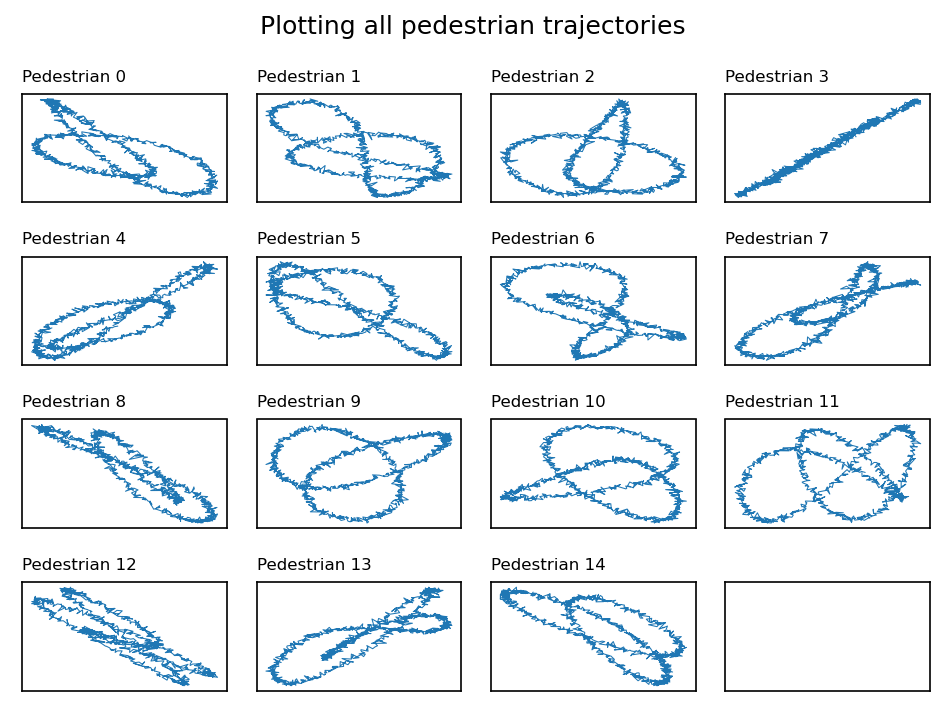
\includegraphics[width=0.7\textwidth]{images_task2/t2_3-allTraj.png}
\caption{All pedestrian trajectories}
\label{fig:t2_3-allTraj}
\end{figure}

\paragraph{3.1: Visualize the path of the first two pedestrians in 2D space}
In Figure \ref{fig:t2_3-pedTraj} we see the trajectories of the first 2 pedestrians from the \verb|data_DMAP_PCA_vadere| data set.
\begin{figure}[H]
\centering
\subfigure[First pedestrian]{
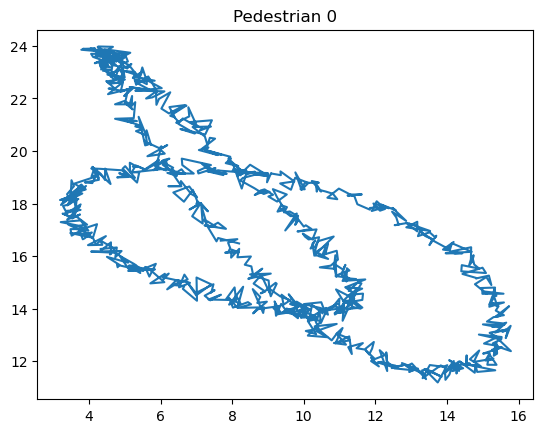
\includegraphics[width=0.4\textwidth]{images_task2/t2_3-ped0.png}}
\subfigure[Second pedestrian]{
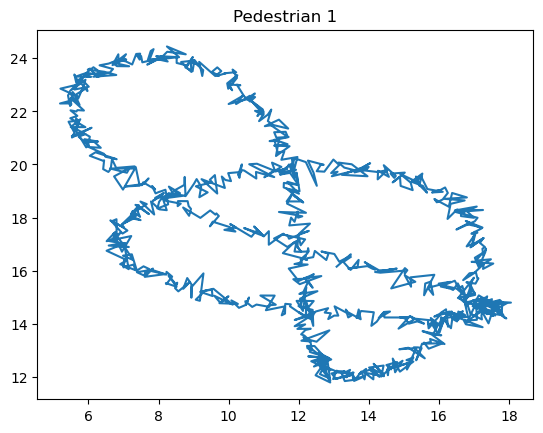
\includegraphics[width=0.4\textwidth]{images_task2/t2_3-ped1.png}}
\caption{2 pedestrian trajectories}
\label{fig:t2_3-pedTraj}
\end{figure}

\paragraph{3.2: Are $l=2$ eigenfunctions $\phi_l$ enough to capture the manifold of the data?}
As seen in Figure \ref{fig:t2_3-allTraj} or \ref{fig:t2_3-pedTraj} we concluded that the pedestrian trajectories are circles. Therefore the diffusion map embedding should result in an ellipse. In Figure \ref{fig:t2_3-dmap} we see that the first two eigenfunctions $\phi_1$ and $\phi_2$ capture the ellipse. Therefore 2 eigenfunctions $\phi_l$ are enough to capture the manifold contained in the pedestrian trajectory.

\begin{figure}[H]
\centering
\subfigure[$\phi_1$ - $\phi_2$]{
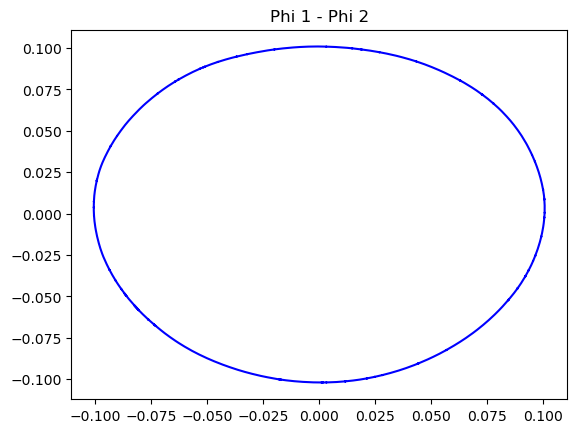
\includegraphics[width=0.35\textwidth]{images_task2/t2_3-phi2.png}}
\subfigure[$\phi_1$ - $\phi_3$]{
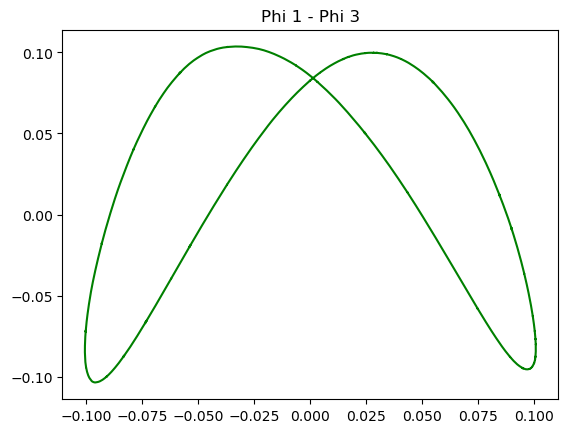
\includegraphics[width=0.35\textwidth]{images_task2/t2_3-phi3.png}}
\subfigure[$\phi_1$ - $\phi_4$]{
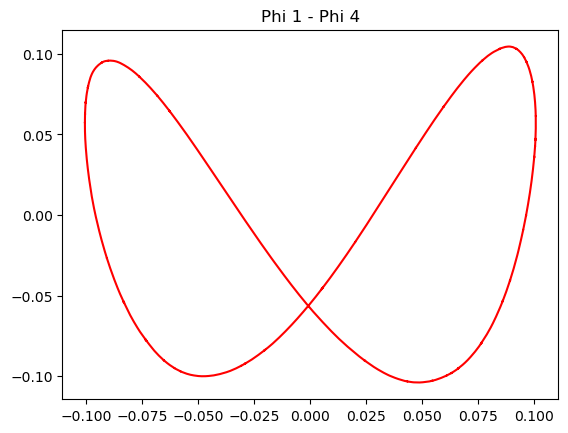
\includegraphics[width=0.35\textwidth]{images_task2/t2_3-phi4.png}}
\subfigure[$\phi_1$ - $\phi_5$]{
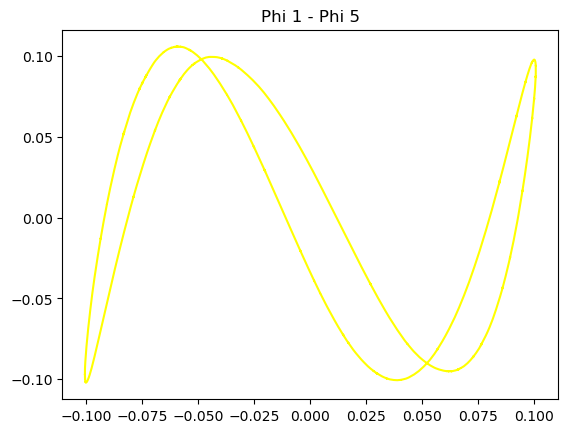
\includegraphics[width=0.35\textwidth]{images_task2/t2_3-phi5.png}}
\caption{Diffusion Map results}
\label{fig:t2_3-dmap}
\end{figure}

\paragraph{3.3: Why, or why not? How many do you need to capture most data set?}
The first 2 eigenfunctions are enough to capture the pedestrian trajectory, because this trajectory \ref{fig:t2_3-pedTraj} boils down to walking in a "circle". The diffusion map unfolds that trajectory into an ellipse, which in Figure \ref{fig:t2_3-dmap}(a) is roughly a circle when considering the values on coordinate axes.

%%%%%%%%%%%%%%%%%%%%%%%%%%%%%%%%%%%%%%%%%%%%%%%%%%
%%%%%%%%%% PART 4
%%%%%%%%%%%%%%%%%%%%%%%%%%%%%%%%%%%%%%%%%%%%%%%%%%
\paragraph{Answering the three questions from the first page of the exercise sheet}
\begin{itemize}
    \item (a) an estimate on how long it took you to implement and test the method. About 12h.
    \item (b) how accurate you could represent data and what measure of accuracy you used. According to \cite{berry2013} we measure accuracy of diffusion maps by compare the diffusion distance against the euclidean distance of the diffusion map embedding. Formally:
    \begin{align*}
        &D_t (x_i ,x_j ) ^2 \approx ||\Phi_{\alpha ,t}(x_i ) -\Phi_{\alpha ,t}(x_j )||_2^2\\
       \Rightarrow &|D_t (x_i ,x_j ) - ||\Phi_{\alpha ,t}(x_i ) -\Phi_{\alpha ,t}(x_j )||_2^2 | < \delta
    \end{align*}
    We follow \cite{roozemond2021} for estimating the accuracy using the mean squared error. Accuracy calculations can found in the python notebooks right after fitting the data. All results are within expectations:
    \begin{center}
    \begin{tabular}{ |c|c|c|c|c|c| }
    \hline
     Test & Fourier ($\phi_1 ,\phi_2$) & SR 5k ($\phi_1 ,\phi_5$) & SR 1k ($\phi_1 ,\phi_5$) & SRD 5k ($\phi_1 ,\phi_5$) & Vadere ($\phi_1 ,\phi_2$)\\
    \hline
     MSE & $0.799$ & $14.976$ & $14.914$ & $14.992$ & $25.197$\\ 
    \hline
    \end{tabular}

    ("SR" - swiss roll with sample size, "SRD" for swiss roll using datafold with sample size)
    \end{center}
    \item (c) what you learned about both the data set and the method (which is probably different from what the machine learned). As seen from the visualization \ref{fig:t2_3-allTraj} the data seems to contain people walking roughly along some curve. Diffusion maps work extremely well in discovering in the underlying manifold, which is an ellipse (or maybe a circle).
\end{itemize}

\end{task}